\documentclass{article}

\usepackage[utf8]{inputenc}
\usepackage[T1]{fontenc}
\usepackage[margin=2.5cm]{geometry}
\usepackage{graphicx}
\usepackage{hyperref}
\usepackage{amsmath}
\usepackage{amssymb}
\usepackage{booktabs}
\usepackage{verbatim}
\usepackage{float}

\graphicspath{{../img/}}

\begin{document}

\title{Lab 5 - Matrix Diagonalization Using the Power Method and Gram--Schmidt Orthogonalization\\
\large{Numerical Methods in Physics}}
\author{Kamil Śmigielski}

\maketitle

\section{Introduction}

The goal of this lab was to write our own C++ program that finds all eigenvalues and eigenvectors of a real
symmetric matrix.
\begin{equation}
    A x_k = \lambda_k x_k .
\end{equation}
We find them with the \emph{Power Method}, and we use \emph{Gram--Schmidt orthogonalization} to get all six
different eigenvectors instead of only the first one. After that, we use the results to rebuild the matrix and
to compute its inverse, and we check how accurate everything is.

\section{The matrix}

The matrix comes from the approximation for a second derivative on equally spaced points,
\begin{equation}
    \left.\frac{d^2 f}{dx^2}\right|_{x_i} \approx \frac{f_{i-1} - 2f_i + f_{i+1}}{\Delta^2},
\end{equation}
with step $\Delta = 1$ and $f = 0$ outside the grid. For $n = 6$ points this gives
\begin{equation}
A = \begin{pmatrix}
-2 & 1 & 0 & 0 & 0 & 0\\
1 & -2 & 1 & 0 & 0 & 0\\
0 & 1 & -2 & 1 & 0 & 0\\
0 & 0 & 1 & -2 & 1 & 0\\
0 & 0 & 0 & 1 & -2 & 1\\
0 & 0 & 0 & 0 & 1 & -2
\end{pmatrix}.
\end{equation}
In the program the matrix is stored as a flat \texttt{double} array of size $n \times n$ and
indexed as \texttt{matrix[n*i + j]}, so row major.

For this matrix the exact answer is known, so we can compare against it:
\begin{equation}
    \lambda_j = -2 + 2\cos\!\left(\frac{j\pi}{n+1}\right), \qquad
    (x_j)_i = \sin\!\left(\frac{i j \pi}{n+1}\right), \qquad i, j = 1,\dots,n .
\end{equation}

\section{Method}

\subsection{Basic tools}
Functions such as the dot product, vector norm, normalization, matrix-vector multiplication, the outer product $q q^T$ and the matrix-matrix product.

\subsection{Power Method}
We start with a nonzero vector $x^{(0)}$ (we used $x^{(0)}_i = i$, i.e.\ $(0,1,2,3,4,5)^T$). In each step we
multiply by $A$ and normalize:
\begin{equation}
    y^{(k)} = A x^{(k)}, \qquad x^{(k+1)} = \frac{y^{(k)}}{\|y^{(k)}\|_2}.
\end{equation}
Each multiplication makes the part of the vector along the eigenvector with the largest $|\lambda|$ grow
faster than all the other parts, so after many steps that direction overwhelms. Normalizing just stops the numbers from
blowing up or shrinking to zero. To read off the eigenvalue we use the Rayleigh quotient
\begin{equation}
    R(x) = \frac{x^T A x}{x^T x}.
\end{equation}

\subsection{Gram--Schmidt}
The plain Power Method always finds the same (dominant) eigenvector. To find the next one, we remove from the
vector every piece that points along the eigenvectors $q_0, \dots, q_{k-1}$ we already have:
\begin{equation}
    y \leftarrow y - \sum_{m=0}^{k-1} (q_m^T y)\, q_m .
\end{equation}
After this the vector is perpendicular to all earlier eigenvectors, so the Power Method is forced to find the
largest of the \emph{remaining} eigenvalues. It must be done each loop as to avoid rounding errors. The core loop of our program is:

\begin{verbatim}
for(int i=0;i<MAX_RECURSION;i++){
  matrixVectorMult(v,matrix.data());
  for(auto vector : eigenvectors){            // Gram-Schmidt
    double scaling_factor = dotProd(v,vector.data());
    for(int i=0;i<LDA;i++){
      v[i] -= scaling_factor * vector[i];
    }
  }
  eigen_stream<<rayleighQuotient(v,matrix.data())<<",\n";
  normalize(v);
}
\end{verbatim}

\subsection{Reconstruction and inverse}
Once we have all normalized eigenvectors $q_k$ and eigenvalues $\lambda_k$, a symmetric matrix can be written
as a sum of simple pieces (the spectral decomposition):
\begin{equation}
    A_{num} = \sum_{k=0}^{5} \lambda_k\, q_k q_k^T, \qquad
    A^{-1}_{num} = \sum_{k=0}^{5} \frac{1}{\lambda_k}\, q_k q_k^T .
\end{equation}
The inverse formula works because none of our eigenvalues is zero.

\subsection{Settings}
We used $n = 6$, $\Delta = 1$, $\mathrm{it}_{max} = 150$ and the tolerance $\varepsilon = 10^{-8}$.
Each eigenvalue is iterated until the residual $\|Ax - \lambda x\|_2$ drops below $\varepsilon$ (or the
iteration cap is reached), and every estimate is saved to \texttt{data/eigenvalue1.txt} \dots\
\texttt{eigenvalue6.txt}.
We then used these files to check when the change between two steps first dropped below $\varepsilon$ (manually).
(Table~\ref{tab:eig}). All plots were made with \texttt{plot/main.py}.

\section{Results}

\subsection{Eigenvalues}

\begin{table}[H]
\centering
\begin{tabular}{cccccc}
\toprule
$k$ & computed $\lambda_k$ & exact $\lambda_k$ & error after 150 it. & $|\lambda_{k+1}/\lambda_k|$ & it.\ until $|\Delta\lambda| < 10^{-8}$ \\
\midrule
1 & $-3.80193774$ & $-3.80193774$ & $1.8\times10^{-15}$ & 0.854 & 56 \\
2 & $-3.24697960$ & $-3.24697960$ & $3.1\times10^{-15}$ & 0.753 & 35 \\
3 & $-2.44504187$ & $-2.44504187$ & $1.3\times10^{-15}$ & 0.636 & 21 \\
4 & $-1.55495813$ & $-1.55495813$ & $1.1\times10^{-15}$ & 0.484 & 15 \\
5 & $-0.75302040$ & $-0.75302040$ & $2.2\times10^{-16}$ & 0.263 & 8 \\
6 & $-0.19806226$ & $-0.19806226$ & $3.1\times10^{-16}$ & -- & 2 \\
\bottomrule
\label{table:eigenvalues}
\end{tabular}
\caption{Computed and exact eigenvalues, ordered from largest to smallest $|\lambda|$.}
\label{tab:eig}
\end{table}

All six eigenvalues agree with the exact formula to about $10^{-15}$, which is the limit of
\texttt{double} precision. All of them settle well before the 150-iteration cap, so the cap was enough for
$n = 6$.

\begin{figure}[H]
    \centering
    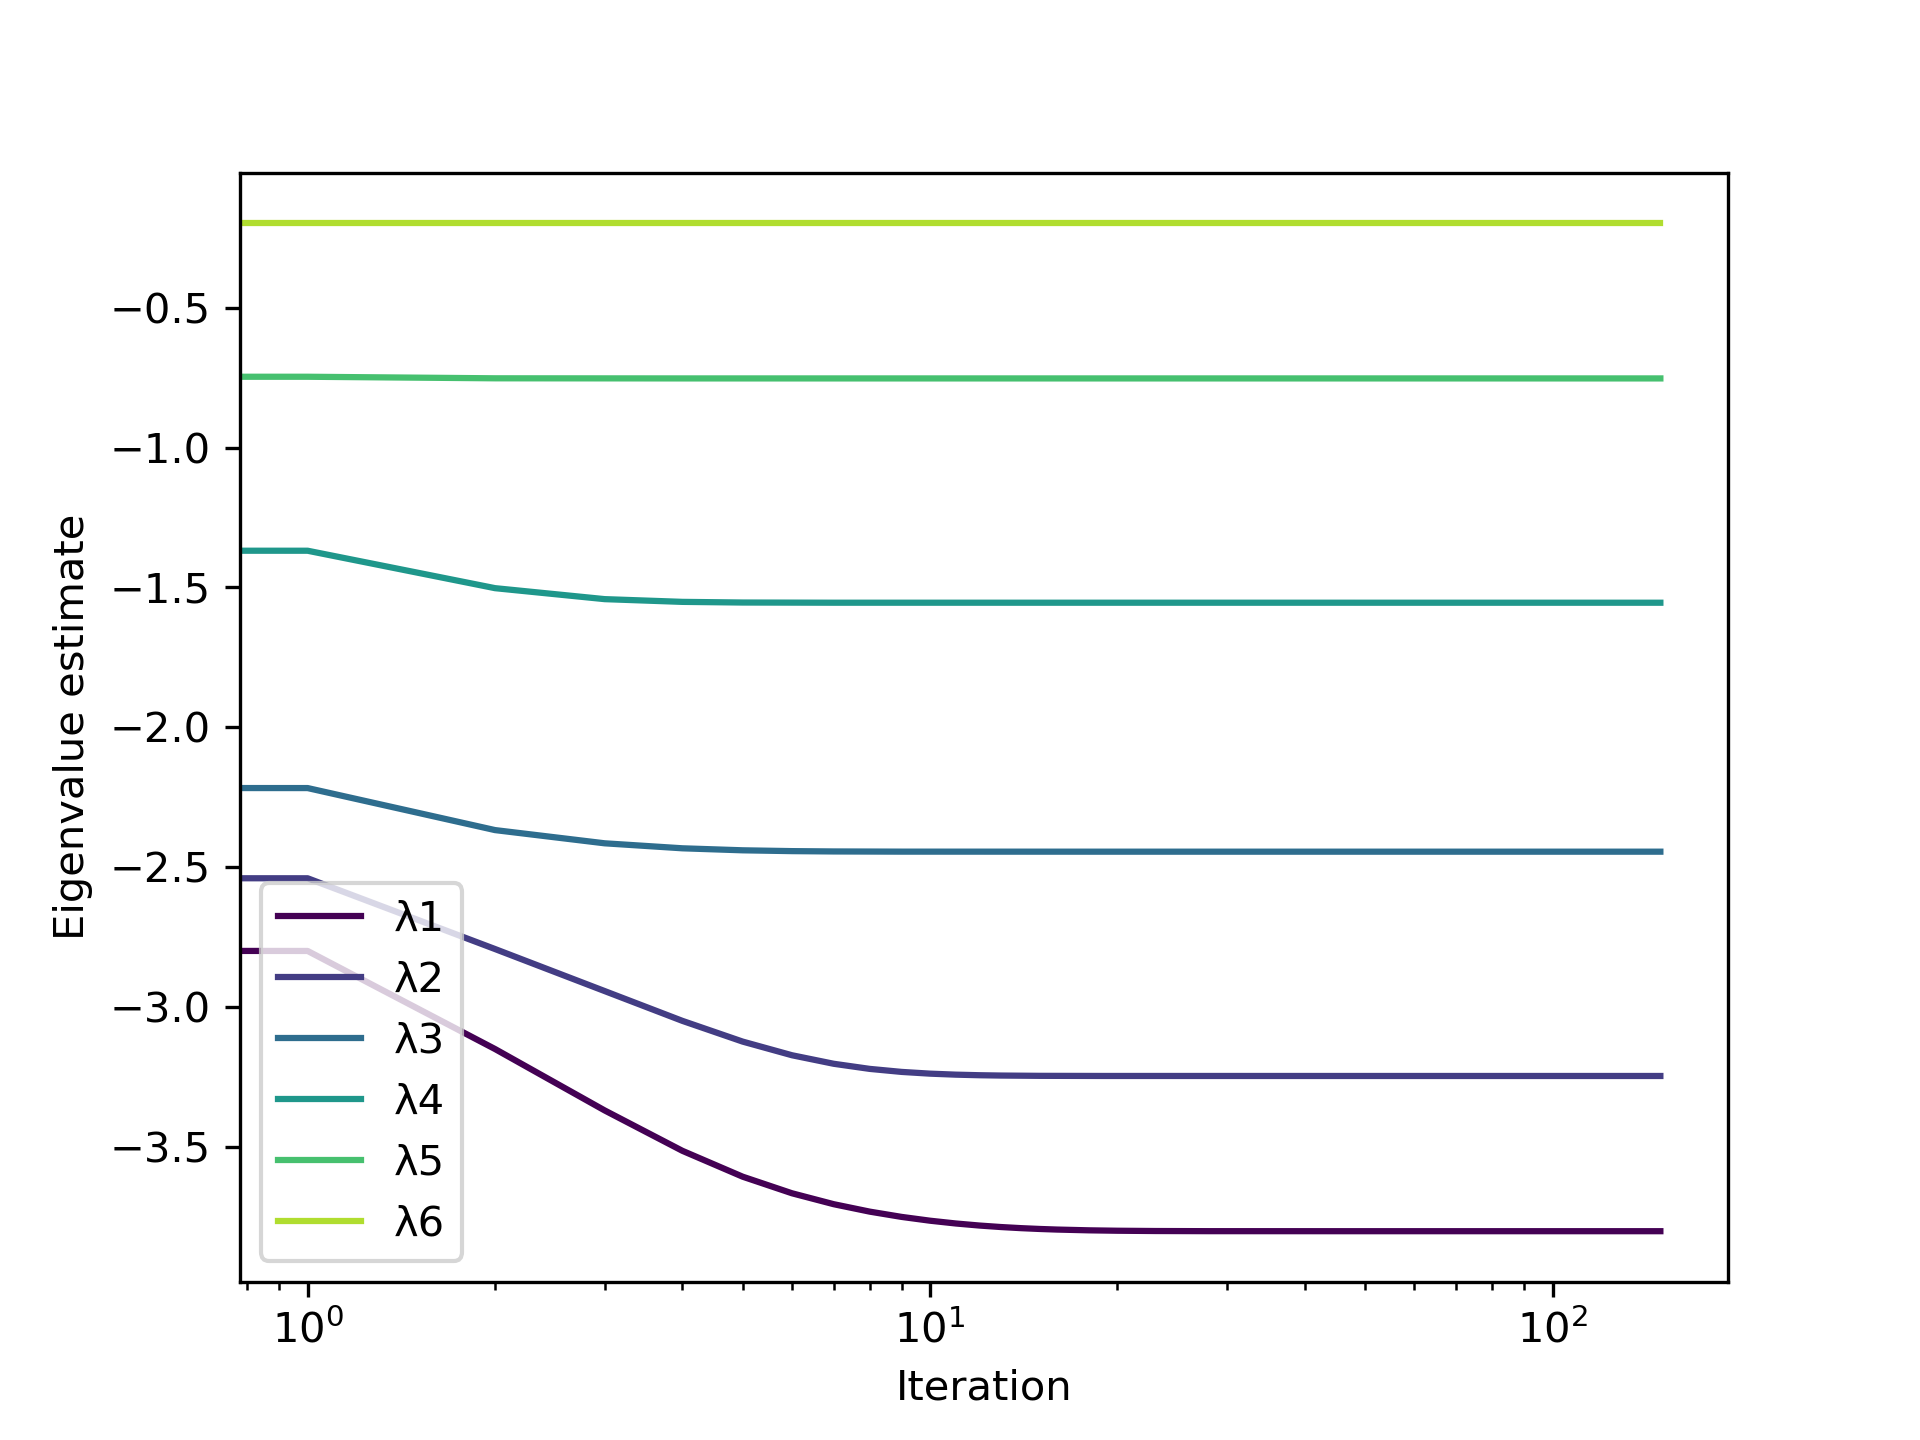
\includegraphics[width=0.85\textwidth]{eigenvalue_history.png}
    \caption{Eigenvalue estimates vs iteration (log scale on the x axis).}
    \label{fig:history}
\end{figure}

\begin{figure}[H]
    \centering
    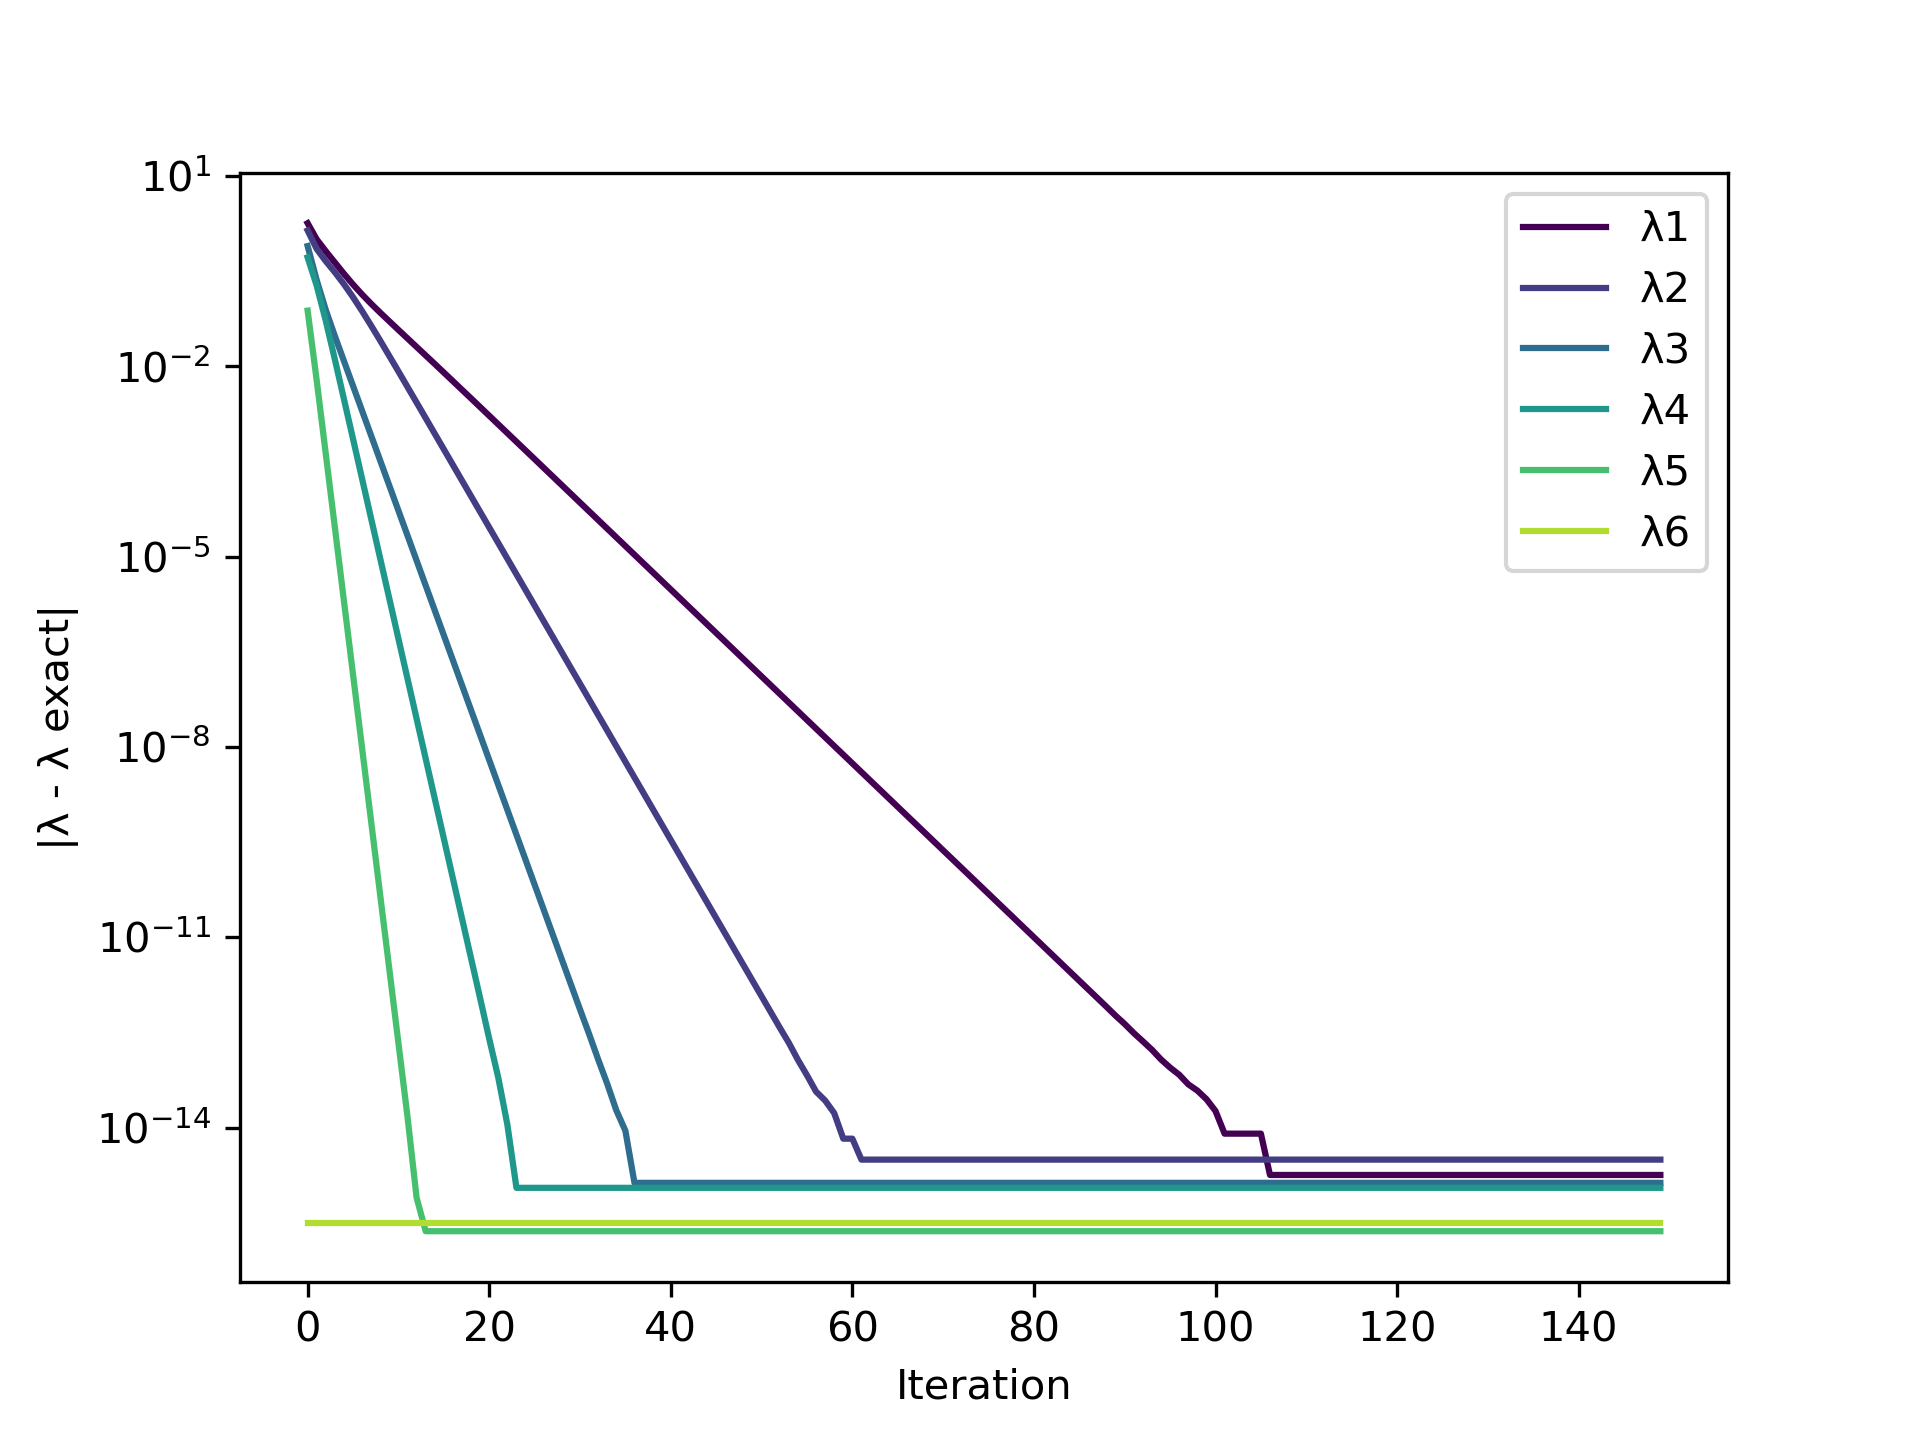
\includegraphics[width=0.85\textwidth]{eigenvalue_error.png}
    \caption{Distance from the exact eigenvalue vs iteration.}
    \label{fig:error}
\end{figure}

\subsection{How fast does each eigenvalue converge?}

Figures~\ref{fig:history} and~\ref{fig:error} show that the eigenvalues found \emph{later} converge
\emph{faster}. After Gram--Schmidt removes the eigenvectors we already found, the
biggest ``competitor'' of $\lambda_k$ is the next one, $\lambda_{k+1}$. Each step shrinks the unwanted part of
the vector by the factor $|\lambda_{k+1}/\lambda_k|$, and the Rayleigh quotient error shrinks by the square of
that factor. On the log plot this gives straight lines, and steeper lines mean smaller ratios.

\textbf{Is this ordering universal?} No. Depending on chosen guess vector, the vector will align with a specific eigenvector, the 
$basis eigenvector$ which is most aligned.

\subsection{Eigenvectors}

\begin{figure}[H]
    \centering
    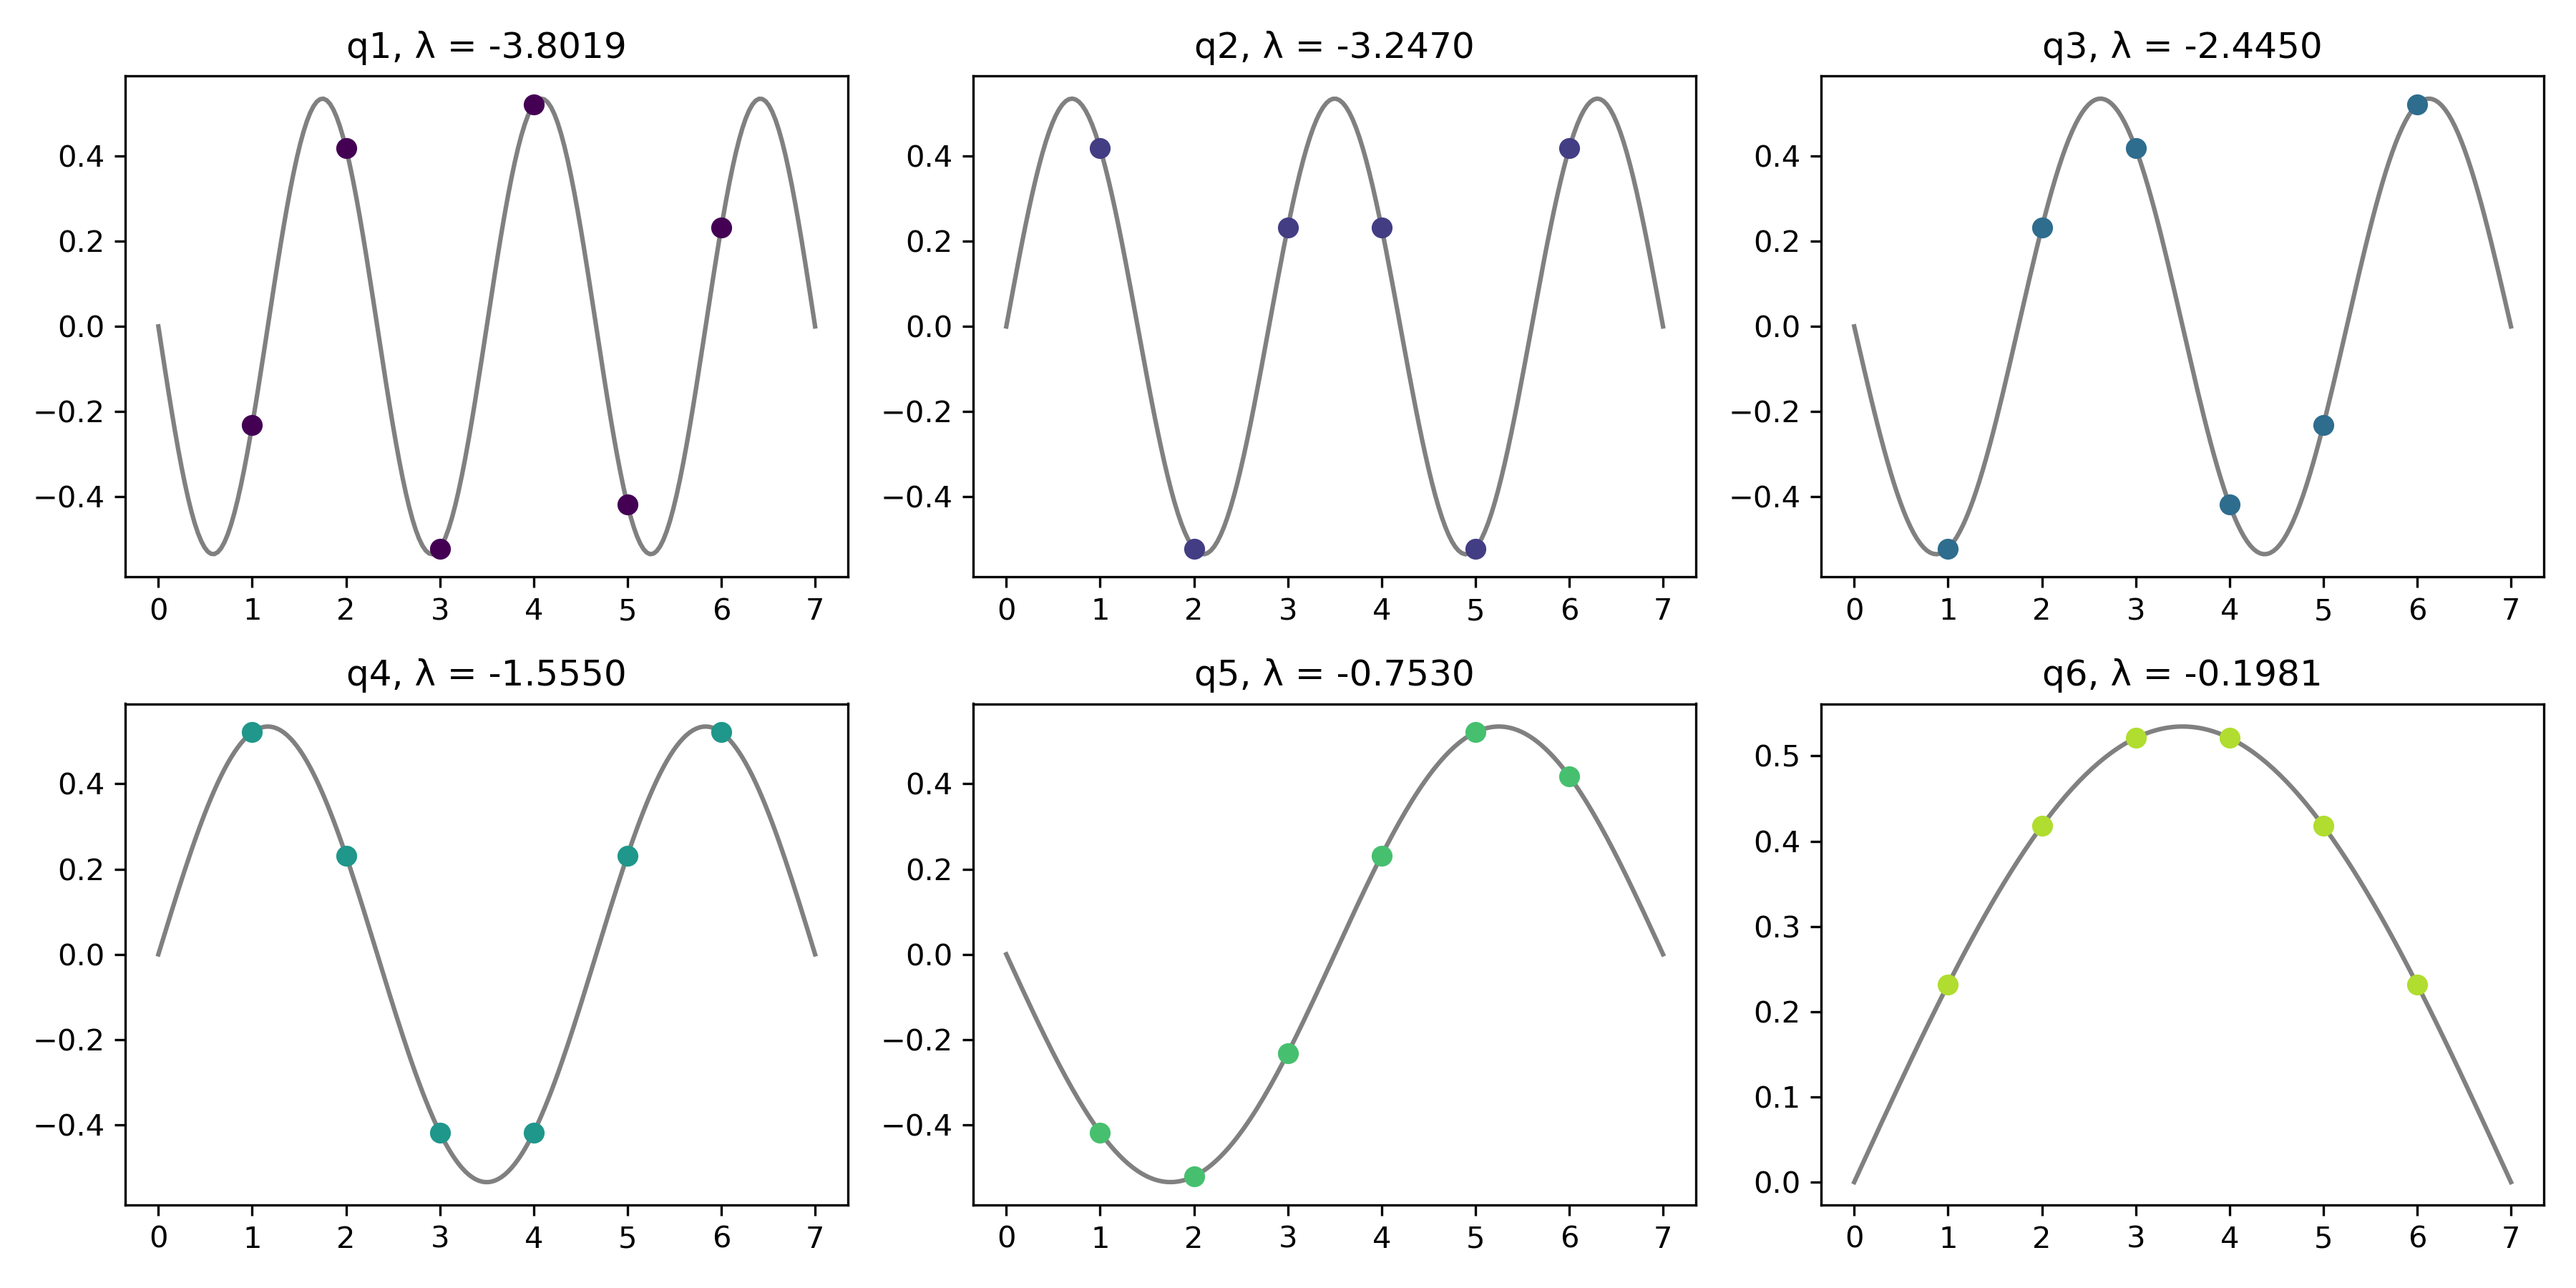
\includegraphics[width=\textwidth]{eigenvectors.png}
    \caption{Computed eigenvectors (dots) and the exact sine curves (grey lines).}
    \label{fig:vectors}
\end{figure}

The computed eigenvectors (Figure~\ref{fig:vectors}) sit exactly on the sine curves. They look like the
standing waves of a string fixed at both ends. The eigenvalue closest to zero ($\lambda_6$) is the smooth
``one-bump'' wave, and the most negative one ($\lambda_1$) is the most wiggly wave, whose sign flips at every
grid point. An eigenvector is only defined up to its sign, so some of ours are flipped compared to the formula;
this does not matter.

\subsection{Checks: residuals, orthogonality, reconstruction and inverse}
The program itself prints the rebuilt matrix (it matches $A$ exactly to the shown digits) and the inverse:
\begin{equation}
A^{-1}_{num} \approx
\begin{pmatrix}
-0.857 & -0.714 & -0.571 & -0.429 & -0.286 & -0.143\\
-0.714 & -1.429 & -1.143 & -0.857 & -0.571 & -0.286\\
-0.571 & -1.143 & -1.714 & -1.286 & -0.857 & -0.429\\
-0.429 & -0.857 & -1.286 & -1.714 & -1.143 & -0.571\\
-0.286 & -0.571 & -0.857 & -1.143 & -1.429 & -0.714\\
-0.143 & -0.286 & -0.429 & -0.571 & -0.714 & -0.857
\end{pmatrix},
\end{equation}
This is indeed the inverse matrix, and the code checks it aswell. 
Multiplying it by $A$ gives the identity matrix (with neglegable 0 sign deviations, stemming from double encoding) to all printed digits.

\section{Discussion}

\subsection{Looser tolerance $\varepsilon = 10^{-4}$}
The eigenvector run for lesser tolerance was approximated directly from generated data of higher accuracy, and the accuracy requirement was 
directly applied from the generated data files, and presented prior in Table ~\ref{table:eigenvalues}.

\subsection{Why the inverse of a symmetric matrix is symmetric}
For any invertible matrix, transposing and inverting can be done in either order: $(A^{-1})^T = (A^T)^{-1}$.
This is because $A^T (A^{-1})^T = (A^{-1} A)^T = I^T = I$. If $A$ is symmetric, $A^T = A$, so
\begin{equation}
    (A^{-1})^T = (A^T)^{-1} = A^{-1}.
\end{equation}

\subsection{Larger matrix, $n = 200$}
Our current data is only for $n = 6$, but by changing the predefined macro's, the simulation yielded a convergence for $\lambda_{1}$ in $\approx 12000$ loops and $\lambda_{6}$ in $\approx 4200$.
\subsection{Turning off Gram--Schmidt}
This experiment yielded the expected conclusion of all eigenvalues converging upon the greatest eigenvalue, being $\lambda_{1} \approx -3.8$
\section{Conclusion}

Our own C++ implementation of the Power Method with Gram--Schmidt orthogonalization found all six eigenpairs of
the $6\times6$ second-derivative matrix. The eigenvalues match the exact formula to about $10^{-15}$ and the
eigenvectors match the expected sine modes. The convergence speed of each eigenvalue is controlled by the ratio
$|\lambda_{k+1}/\lambda_k|$, so for this matrix the later eigenvalues converge faster; this order is not
universal. Using the eigenpairs we rebuilt $A$ and computed $A^{-1}$, and both pass the checks
($A_{num}\approx A$, $AA^{-1}_{num}\approx I$) up to the precision of the saved data. Finally, the method only
works well when the eigenvalues are well separated and Gram--Schmidt is applied in every step.

\end{document}
